\section{Modelling}

\subsection{Single Compressor}
\begin{frame}{Compressor Model}
  \begin{minipage}{0.6\linewidth}
    \resizebox{\linewidth}{!}{
      \begin{tikzpicture}
        \drawcomp
      \end{tikzpicture}
    }
  \end{minipage}
  \begin{minipage}{0.38\linewidth}
  \begin{itemize}
    \item Atmospheric pressure at boundary
    \item Controlled inputs: \g{ur} and \g{torque}
    \item Outputs: \g{sd} and \g{pd}
  \end{itemize}
\end{minipage}
  % What model is used for the compressor?\\
  % Where does it come from?\\
  % What are the significant non-linearities?\\
  % Inputs/outputs/states
\end{frame}

\begin{frame}{Surge Distance}
    \centering
    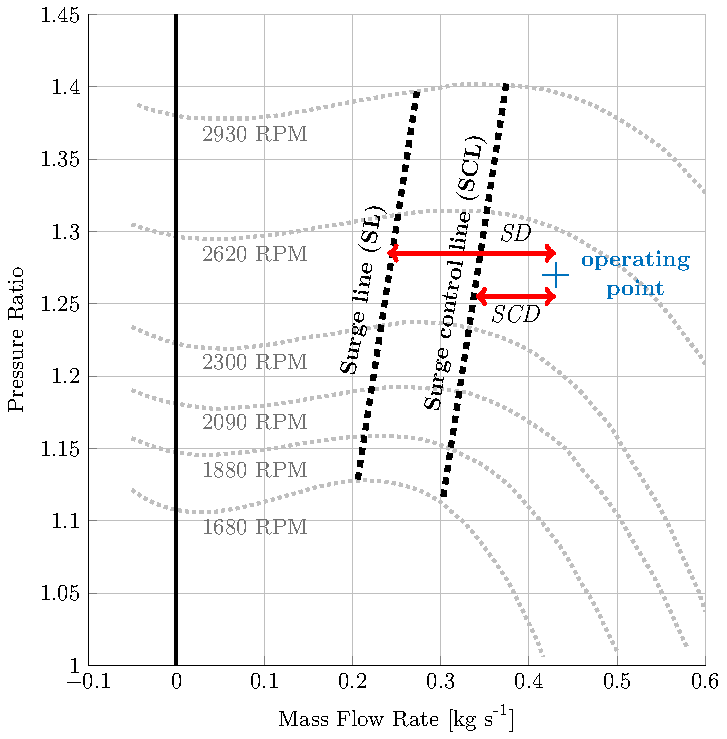
\includegraphics[width=.5\linewidth]{figures/surge.pdf}
\end{frame}

\subsection{Compressor Systems}

\begin{frame}{Parallel System}
    \centering
    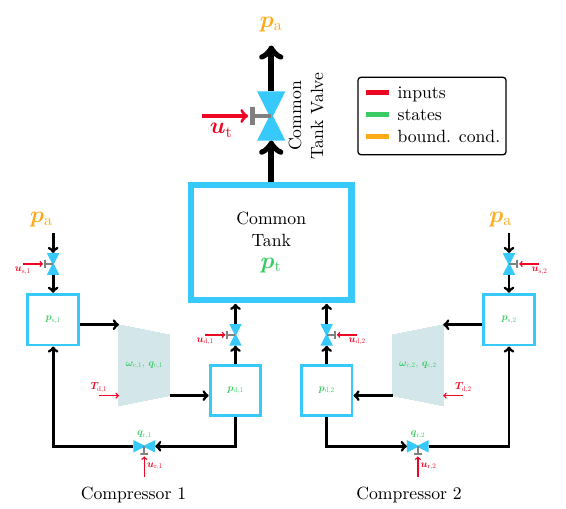
\includegraphics[width=.7\linewidth]{modelling/diagram_parallel.png}
\end{frame}

\begin{frame}{Serial System}
    \centering
    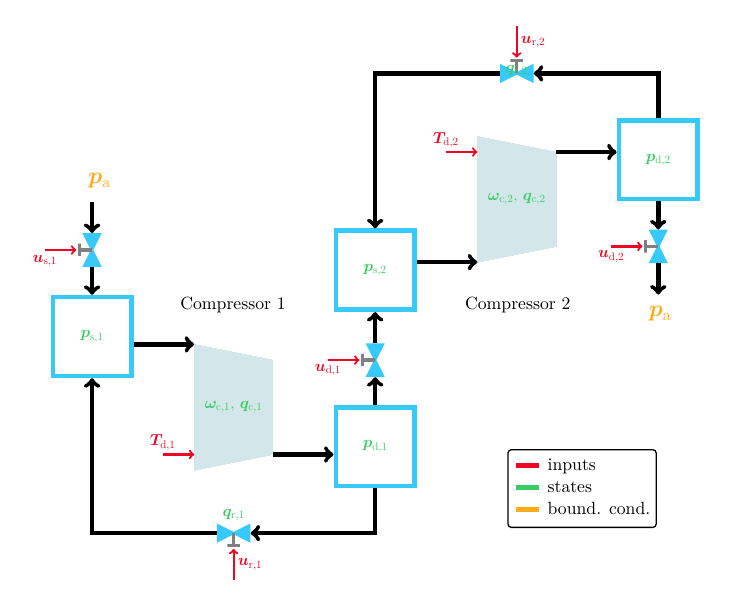
\includegraphics[width=.7\linewidth]{modelling/diagram_serial.png}
\end{frame}

